%%%%%%%%%%%%%%%%%%%%%%%%%%%%%%%%%%%%%%%%%
% iConference Article
% LaTeX Template
% Version 2.1 (25/10/13)
%
% This template has been downloaded from:
% http://www.LaTeXTemplates.com
%
% Original author:
% Frits Wenneker (http://www.howtotex.com)
%
% Modified by:
% Joseph Helsing (2012)
% Heinz-Alexander Fütterer, Maxi Kindling, Stephanie van de Sandt (2013)
% Cory Knobel (2014)
%
% License:
% CC BY-NC-SA 3.0 (http://creativecommons.org/licenses/by-nc-sa/3.0/)
%
%%%%%%%%%%%%%%%%%%%%%%%%%%%%%%%%%%%%%%%%%

%----------------------------------------------------------------------------------------
%	LIST OF NECESSARY PACKAGES
%----------------------------------------------------------------------------------------

% The packages used in this template were: fontenc, babel, microtype, indentfirst,
% geometry, multicol, graphicx, apacite, caption, booktabs, float, footnote, paralist,
% titlesec, fancyhdr, xcolor, tabularx, lipsum

%----------------------------------------------------------------------------------------
%	PACKAGES AND OTHER DOCUMENT CONFIGURATIONS
%----------------------------------------------------------------------------------------
\documentclass[10pt, letterpaper]{article}
\usepackage[T1]{fontenc} % Use 8-bit encoding that has 256 glyphs
\usepackage{lmodern}
\usepackage[english]{babel}
\linespread{1.05} % Line spacing - Palatino needs more space between lines
\usepackage{microtype} % Slightly tweak font spacing for aesthetics
\setlength{\parindent}{0.5in} % Indent 0,5 inch
\usepackage[top=.8in, bottom=0.8in, left=1in, right=1in]{geometry} % Document margins
\usepackage{graphicx}
\usepackage{xcolor}
\usepackage[implicit=false,colorlinks=true,allcolors={black},urlcolor={black}]{hyperref}

\usepackage{apacite} % Allows for the correct APA citation of references
\renewcommand{\bibliographytypesize}{\fontsize{10pt}{10pt}} % Set the bibliography font size to 10pt

\usepackage{url}
\usepackage{tabularx}
\usepackage{booktabs} % Horizontal rules in tables
\usepackage[sf]{titlesec} % Font of Headings

\usepackage[normal]{caption} % Custom captions under/above floats in tables or figures
\captionsetup{format=plain,justification=RaggedRight,singlelinecheck=false}
\usepackage{footnote} %Enables footnotes

\makeatletter
\def\blfootnote{\selectfont\xdef\@thefnmark{}\@footnotetext}
\makeatother %This is used to allow for blank footnotes

\usepackage{paralist} % Used for the compactitem environment which makes bullet points with less space between them

\usepackage{fancyhdr} % Headers and footers
\pagestyle{fancy} % All pages have headers and footers
\fancyhf{}
\fancyhead[L]{\vspace{-15mm}\fontsize{10pt}{10pt}\selectfont{iConference 2016} }%This is the header
\fancyhead[R]{\vspace{-15mm}\fontsize{10pt}{10pt}\selectfont{[Burton]} }
\fancyfoot[C]{\thepage} % Custom footer text

\usepackage{tocloft} % Change List of Figures / Tables
\renewcommand{\cftfigpresnum}{Figure }
\setlength{\cftfignumwidth}{5em}
\renewcommand{\cfttabpresnum}{Table }
\setlength{\cfttabnumwidth}{5em}
\renewcommand\cftloftitlefont{\sffamily \Large}
\renewcommand\cftlottitlefont{\sffamily \Large}

%----------------------------------------------------------------------------------------
%	TITLE SECTION
%----------------------------------------------------------------------------------------

\title{Looking for the Core: Preliminary Explorations of iCaucus Syllabi}

%----------------------------------------------------------------------------------------

\date{} % no date

% Formatting title and authors.
\makeatletter
\renewcommand{\maketitle}{\bgroup\setlength{\parindent}{0pt}
\begin{flushleft}
  {\sffamily \Large {\@title} }
  \vspace{12pt}\\
  \@author
\end{flushleft}\egroup
}
\makeatother

%----------------------------------------------------------------------------------------
% AUTHORS
%----------------------------------------------------------------------------------------

\author{%
{\large Matt Burton$^{1}$\\} % Enter authors.
$^{1}$University of Pittburgh\\ % Enter affiliations.
}


%----------------------------------------------------------------------------------------

\begin{document}

\newenvironment{blockquote}{\list{}{\leftmargin=0.5in\rightmargin=0.0in}\item[]}{\endlist}
\renewcommand{\listfigurename}{Table of Figures} 
\renewcommand{\listtablename}{Table of Tables} 
\maketitle % Insert title
\thispagestyle{empty} % First page has no header,footer

%----------------------------------------------------------------------------------------
%	INFOBOX
%----------------------------------------------------------------------------------------

\begin{center}
\begin{tabularx}{\textwidth}{|X|}
\hline
\vspace{2pt}\\
\textbf{Abstract}\\
The purpose of this study is to perform an empirical analysis of existing "core" or "foundation" courses in iSchools to better understand what the community implicitly considers to be its foundational knowledge base. This paper presents a preliminary journal citation analysis of core syllabi from master's programs in the iCaucus. Initial findings show journals from library science and information science dominate the field and only eight articles are cited by more than two courses. Finally, the disciplinary diversity of programs was calculated and visualized showing how interdisciplinarity is expressed across the iCaucus. The hope is that this initial report will help enroll additional collaborators, either as data providers or analysts, and stimulate a data-rich conversation about what we teach in core courses.\\
{\footnotesize \textbf{Keywords:} ischools; interdisciplinary; graduate education; foundations courses}\\
{\footnotesize \textbf{Citation:}  Burton, M. (2016). Looking for the Core: Preliminary Explorations of iCaucus Syllabi. Presented at the IConference 2016 Proceedings, iSchools. http://doi.org/10.9776/16225
}\\
{\footnotesize \textbf{Copyright:} Copyright is held by the authors.}\\
{\footnotesize \textbf{Research Data:}  https://github.com/mcburton/ischools-core} \\ % Please delete line if not used.
{\footnotesize \textbf{Contact:} mcburton@pitt.edu}\\ % Please enter at least one contact e-mail address. 
\vspace{2pt}\\
\hline
\end{tabularx}
\end{center}

%----------------------------------------------------------------------------------------
%	ARTICLE CONTENTS
%----------------------------------------------------------------------------------------
\section{Introduction}
iSchools are sites of diverse faculty, teaching, and epistemologies. As interdisciplinary institutions, iSchools don't necessarily have "core" set of concepts, ideas, methods, and practices rooted in a disciplinary history rather they are an amalgam of disciplinary orientations dedicated to exploring the relationship between information, people, and technology.\footnote{http://ischools.org/about/} While library and information science (LIS) may be the closest thing iSchools have to a disciplinary history, as interdisciplinary institutions they address a much broader body of knowledge and practice. What is the extent of this epistemological diversity? How do iSchools wrestle with the constitution of their core or foundational courses? Every iSchool is faced with the challenge of assembling core courses, but the existing core courses have not been empirically studied in depth.

The purpose of this study is to perform an empirical analysis of the existing "core" or "foundation" courses in iSchools to better understand what the community implicitly considers to be our foundational knowledge base. While the designers of core courses have presumably communicated in and through various invisible colleges, a more explicit and procedural effort to collect, analyze and understand what iSchools consider their core would be a boon for the community. The results of this study hope to inform the practical design of core courses but also provoke a more deliberate, data-rich conversation about our core (or cores) methods, concepts, theories, and practices.

This paper presents very early results of an analysis of core course syllabi from master's programs in the iCaucus.\footnote{http://ischools.org/members/icaucus-members/} The data are incomplete and the analysis has been narrowly scoped. However, there is enough to draw out some initial findings about journals cited in foundations courses and the disciplinary diversity of master's programs. Initial findings show Library Science and Information science are the main disciplinary orientation of iSchools and only eight articles are cited by more than two courses in data collected in time for publication. The hope is that this initial report will help enroll additional collaborators, either as data providers or analysts, and stimulate a conversation about what we teach in core courses.  

\subsection{Research Questions}
This initial research addresses the following research questions using a partial data set of journal citations from the core courses in master's degree programs in the iSchools caucus. This research 
\begin{compactitem}
	\item RQ1: What are the most cited journals in core syllabi?
	\item RQ2: What are the most cited journal articles in core syllabi?
	\item RQ3: How diverse are individual schools and programs?
\end{compactitem}

\section{Background}
There have been a mix of essays and empirical work reflecting upon the character of iSchools. The composition of iSchool faculty has been extensively studied \cite{wiggins_intellectual_2012, holmberg_conceptual_2013, wu_state_2012, chen_thematic_2008} exploring the degree of interdisciplinarity in research interest, funding sources, and collaborators. Looking at faculty is only one of many ways in which we can understand the character of iSchools. What we teach students is another.

There have been several studies of library \cite{subramaniam_weaving_2010, wedgeworth_robert_certain_2013, corrall_educating_2010} and archives curricula \cite{bastian_are_2005, bastian_towards_2006}, but these focus on L-Schools or particular specializations within iSchools. Seadle and Greifeneder \citeyear{seadle_envisioning_2007} explicitly wonder if there should be a curricular distinction between iSchools and library schools. They argue that iSchools should adopt a broader curriculum than LIS, more focused on human-computer interaction.

Wu et al. \citeyear{wu_state_2012} specifically analyzed core courses at the master's and doctoral level, but only used course title and description as their data. They conclude " individual iSchools offer many different degrees: this may be an indication of the diverse disciplinary foundation of each school or it might signify that iSchools are still at the stage of exploring and coping with the changes in the environment in their curricula" \cite[p. 32]{wu_state_2012}.

This empirical research into the foundational curriculum of iSchools has only touched upon the surface of the data available. Now that iSchools have been teaching students for over two decades, there is an opportunity for a data-rich conversation around the core (or cores) of iSchool pedagogy. This project aims stimulate that conversation with an empirical analysis that dives \textit{into} the content of core course syllabi. 

\section{Methods}
Data collection for this study had three phases. The first phase surveyed master's degree programs of schools in the iCaucus. The iCaucus was selected because the 24 schools are a manageable sample size for this initial research. Dual degree programs and programs outside the information disciplines, like education or computer science, were excluded because they represent distinct (although related) disciplines. The second phase enumerated "core" or "foundation" courses for each of the selected degree programs. This effort focused on core courses at the program level, not the core requirements for individual specializations within programs. 

Finally, there is an ongoing effort to obtain a reasonably recent copy of course syllabi. Of the 25 iCaucus schools, syllabi from 14 schools have already been obtained. Syllabi were obtained from institution catalogues, from faculty home pages, or via personal communication. Convenience sampling has guided the collection process with a total of 63 syllabi collected in time for publication.

Citations from a variety of scholarly and non-scholarly sources were extracted from the syllabi. Citation strings were parsed using the web service Anystyle.io,\footnote{http://anystyle.io} which yielded machine readable data structures (author, title, journal, year, etc.). In addition to parsing, Anystyle.io classified citations as \textit{book}, \textit{article}, \textit{incollection}, \textit{inproceeding}, \textit{misc}, or \textit{report}. Additional cleaning was performed by hand and using the OpenRefine\footnote{http://openrefine.org} data cleaning tool.

The top articles and journals titles were compiled to answer RQ1 and RQ2. To answer RQ3, the journal titles were qualitatively coded with one of twenty disciplinary categories (Library Science, Information Science, Economics, Anthropology, etc.). Categories with fewer than 15 instances were aggregated into a set of higher level categories (\textit{Archives, Computer Science, HCI, Humanities, Information Science, Law, LIS, Management, Misc, News, Science, Social Sciences}). These affiliations were used to calculate the disciplinary proportion for each master's degree program by counting the number of journal citations per disciplinary affiliation divided by the total number of journal citations for all citations in an individual program's core syllabi.

\section{Findings}
A total of 1,827 citations were extracted from 63 syllabi from 14 iSchools. 882 citations were classified as journal articles, 400 as books, 220 in collections or book chapters, 90 in conference proceedings, 206 as miscellaneous, and 29 as reports. The findings reported in this article focus on the 882 journal articles from the syllabi collected at the time of publication. Data collection of missing syllabi and analysis of non-journal citations is in-progress.

The sections below answer three research questions: What are the most cited journals in core syllabi? What are the most cited journal articles in core syllabi? and How diverse are individual schools and programs?

\subsection{Top Cited Journals}

\begin{figure}[h]
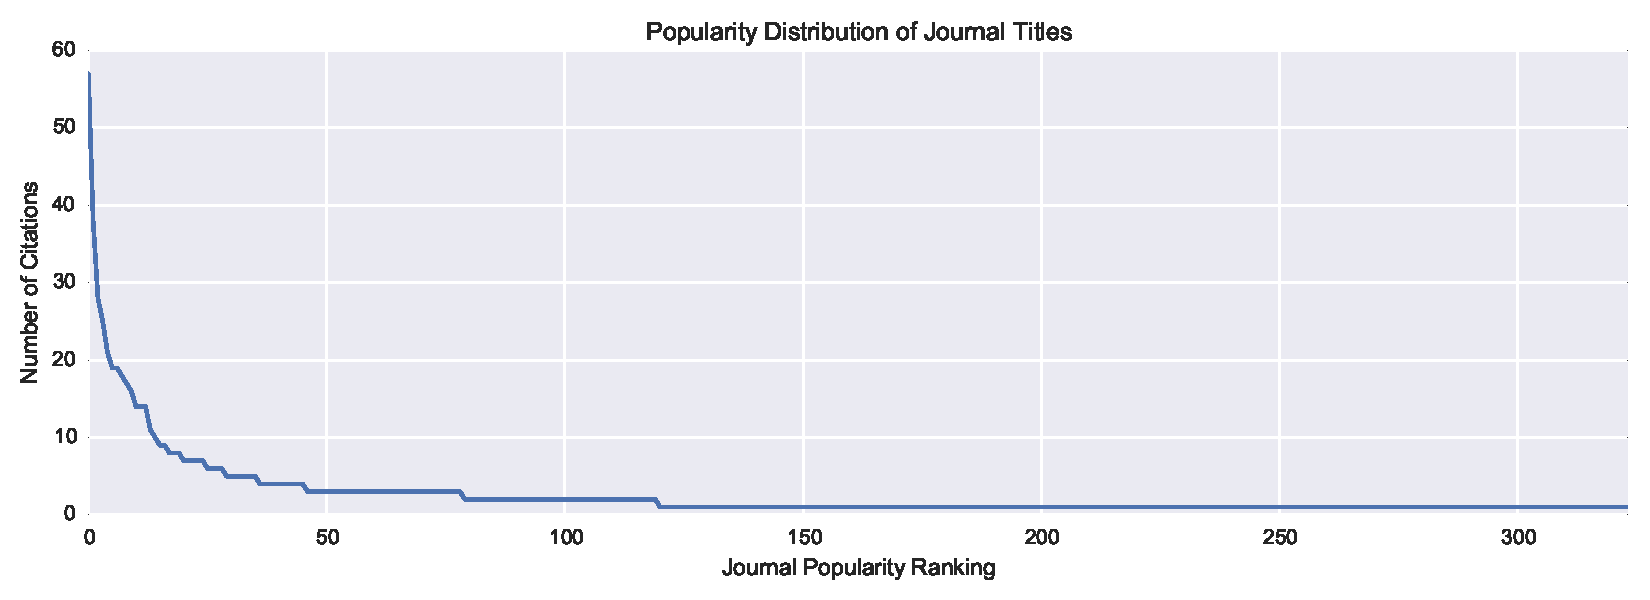
\includegraphics[width=\textwidth]{popular-journals.pdf} 
\caption{Distribution of journal popularity ranked by number of citations.} 
\end{figure}

Out of 882 journal citations, around 340 unique journal titles were identified. Figure 1 shows the distribution of popular journals based on the number of citations within the data. At the left end of the chart a small number of journals are regularly cited more than ten times with a long tail of journals cited only once or twice. The distribution roughly follows a power law distribution or the 80-20 rule where around 80\% of the citations come from only 20\% of the journals. This leads to the question, What specific journals are the most cited in core course syllabi?

\begin{table}[h]

\begin{tabular}{lll}
\toprule
Rank & Title & Count \\
\midrule
1 & \textit{Journal of the American Society for Information Science \& Technology} & 94 \\
2 & \textit{Journal of Documentation} & 28 \\
3 & \textit{Information Processing \& Management} & 19 \\
4 & \textit{Library Trends} & 21 \\
5 & \textit{College \& Research Libraries} & 19 \\
6 & \textit{Harvard Business Review} & 19 \\
7 & \textit{Interactions} & 18 \\
8 & \textit{Journal of Information Science} & 17 \\
9 & \textit{Journal of Academic Librarianship} & 16 \\
10 & \textit{Cataloging \& Classification Quarterly} & 14 \\
\bottomrule
\end{tabular}
\caption{Rank, title, and count of the most popular journals cited in core course syllabi.}
\end{table}

Table 1 lists the top 10 most cited journals in the data collected so far. JASIST and JASIS have been combined to reflect the change in the journal's name in 2001, however both journals occupy the top two spots in the ranking with 57 citations and 37 citations respectively. Journals affiliated with library science accounted for 31\% of the total citations, with information science coming in 2nd place at 24\%. The next highest disciplinary affiliations, management, social sciences, and HCI, each occupied 7\% of the total citations. News represented 6\% and the remaining disciplinary affiliations (humanities, science, misc, computer science, law, and archives) each had less than 5\%.


\subsection{Top Cited Articles}

\begin{figure}[h]
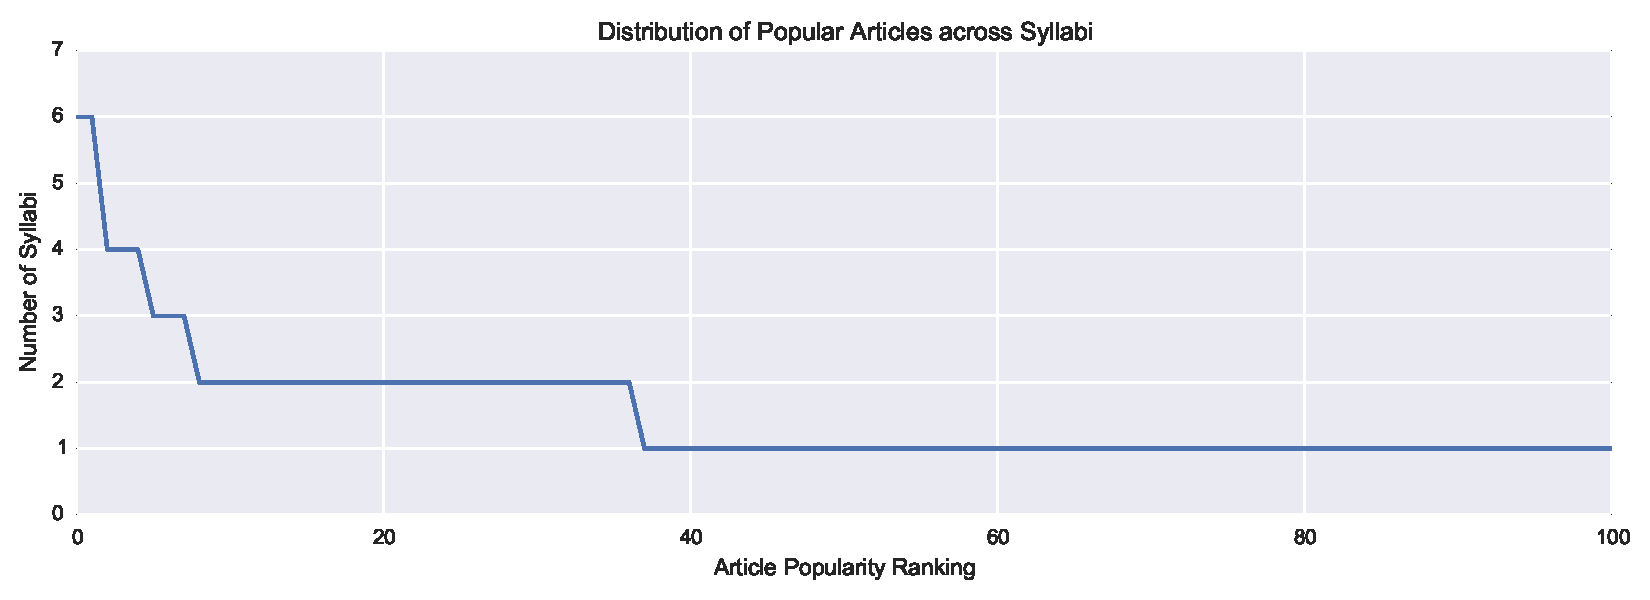
\includegraphics[width=\textwidth]{popular-articles.pdf} 
\caption{Distribution of article popularity ranked by the number of citations.} 
\end{figure}

Figure 2 shows the distribution of popular journal articles in the data. Only eight articles are cited on more than two syllabi. Two citations appear on six syllabi, three citations appear on four syllabi, and three citations appear on three syllabi. These findings indicate a partial overlap of citations at the journal article level. This makes finding a distinct "core" within the iSchools challenging (hence the report of top-ranked journal titles above). There is no one article that is cited in all or nearly all the syllabi across the programs, instead this collection of eight articles represents what could be called a "core-ish" set within the iCaucus core courses. 

\begin{table}[h]

\begin{tabular}{lll} 
\toprule
Rank & Author/Title & Count \\
\midrule
1 & Bush, As We May Think & 6 \\
2 & Buckland, Information as Thing & 6 \\
3 & Bates, The invisible substrate of information science & 4\\
4 & Bates, The design of browsing and berry-picking techniques for online search interface & 4 \\
5 & Elings \& Waibel, Metadata for all & 4 \\
6 & Taylor, Question negotiation and information seeking in libraries & 3 \\
7 & Kuhlthau, Inside the search process: Information seeking from the user's perspective & 3 \\
8 & Buckland, What is a "Document"? & 3 \\
\bottomrule
\end{tabular}
\caption{Rank, title, and count of the most popular articles cited in core course syllabi.} 
\end{table}

Table 2 lists the authors and titles of eight "core-ish" journal citations. These eight articles garnered a total of 30 citations from the total of 882 article citations in the data. These findings also show the most influential authors in the iSchools. Buckland and Bush are tied in first place appearing on 6 syllabi each. Bates appears twice in the ranking of second place authors, Buckland appears again in the third place ranking.

\subsection{Diversity of Programs}
The third research question addresses the degree to which we can empirically measure the interdisciplinarity of iSchool's core curriculum. This was operationalized by counting the disciplinary affiliation of journal citations in the core courses aggregated at the school/program level. Many iSchools have more than one master's program so each program, rather than school, is treated as an independent unit in the analysis. For example, the University of Maryland has three programs in their iSchool, a masters in Library Science (MSLS), a masters in Information Management (MIM), and a masters in Human Computer Interaction (MSHCI). Other iSchools, like the University of Michigan, have a single Masters in Information (MSI).

\begin{figure}[h]
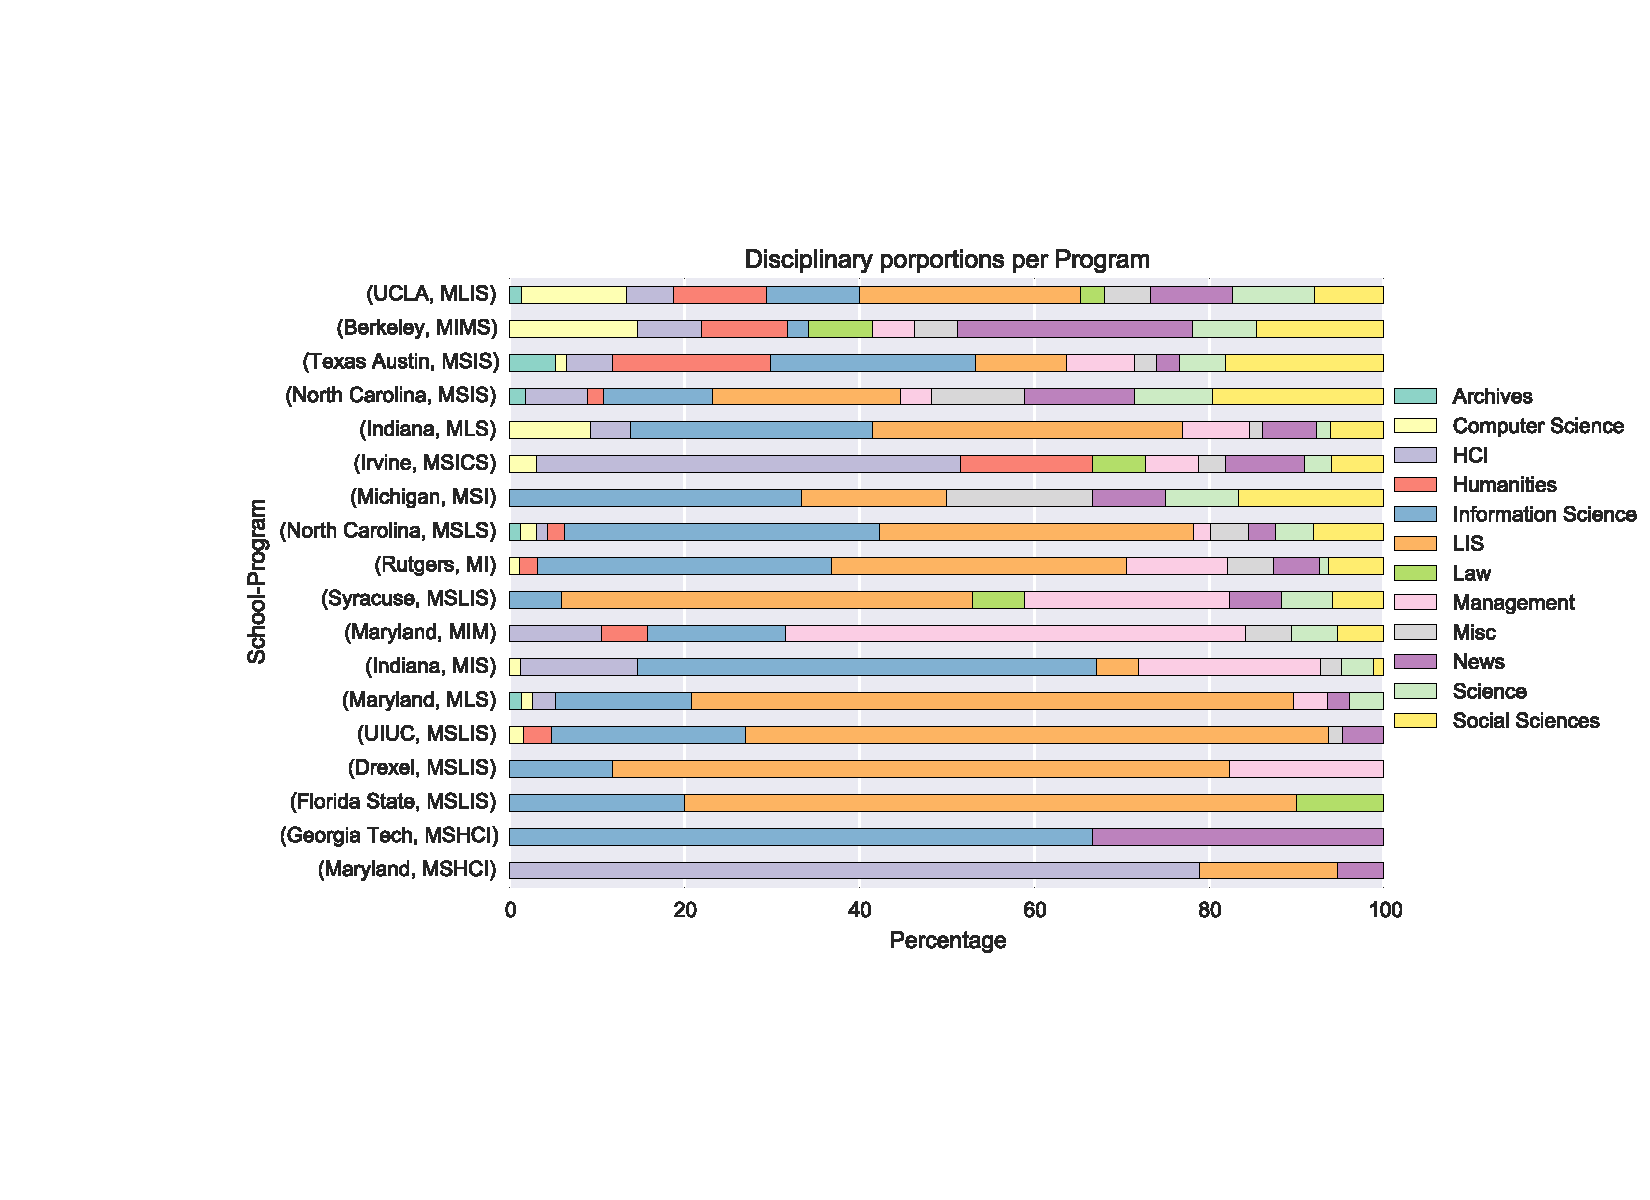
\includegraphics[width=\textwidth]{proportion_per_program.pdf} 
\caption{Proportions of citations per discipline area for each program. Programs are ordered, top to bottom, from most to least diverse.} 
\end{figure}

Figure 3 shows a program's disciplinary diversity as measured by the proportion of disciplines expressed in journal citations for each master's program. Schools are ordered from top to bottom based using entropy as a metric for diversity. Higher entropy yields a more interdisciplinary set of core courses. Programs like UCLA and Berkeley include a diverse selection of journal citations across the 12 disciplinary categories described above. Programs like Maryland's MSHCI, Georgia Tech, and Florida State express a lesser degree of diversity in their core courses.\footnote{One might expect Georgia Tech to have a higher proportion of HCI instead of information science and news, but this doesn't include conference proceedings which are the main venue for HCI research.} Not all programs express each of disciplinary categories, and the total number of citations varies per program.

\section{Discussion \& Conclusion}
It is difficult at this stage of the project to make any definitive claims about the core teaching materials of iSchools. But this analysis of journal articles informs our understanding of what iSchools teach master's students. Library and information science journal citations dominate the subject matter of core syllabi, but the presence of the \textit{Harvard Business Review} and \textit{Interactions} in the list of top ranked journals show management and human computer interaction have a place as well. It should be noted not all syllabi have the same number of citations and could skew the results whereby syllabi with a large number of citations have more voice in aggregate measures. A more nuanced analysis with additional data may reveal further complexity to the interdisciplinary character of the core.

A small number of articles were similarly cited across several schools and programs. Of the top ranked articles, there are three in particular whose expansive scope are effective at orienting the iSchools mission around people, information, and technology. With a bit of alliterative and interpretive flourish, it is argued iSchools cherish the three B's: Buckland's \textit{Information as Thing}, Bate's \textit{The invisible substrate of information science}, and Bush's \textit{As We May Think}. Each article addresses a different facet of iSchools interdisciplinary character, in a clarification of our fundamental object, in an analysis of taken-for-granted disciplinary assumptions, and in a retro-futuristic vision. These three articles in particular set a tone for a kind of big-picture thinking that is crucial for students as they become information professionals.\footnote{It should be noted the context and framing in which these articles are cited within syllabi should be investigated before making an overly strong claim of their significance.}

The iSchools are not uniformly interdisciplinary and each take a different approach to expressing their disciplinary orientation. We should not \textit{definitively} conclude the diversity of a program based journal citations as some core courses are book centric and have yet to be fully analyzed. An iSchool's interdisciplinarity can also be divided across programs rather than contained within a single program. For example, Maryland's human computer interaction program is mostly composed of HCI citations, the library science program is mainly LIS citations, and the management program is mainly management citations. Berkeley has a single program in which they include their interdisciplinary core. As such, the individual diversity of Berkeley's MIMS program is higher than any individual program at Maryland. 

These findings show a wealth of information about the iSchools that has yet to be fully analyzed and interpreted. This paper presents very preliminary findings about the syllabi of core courses in the iCaucus. This analysis focused its attention upon 882 journal articles, at the expense of 400 books, 220 book chapters, 90 conference proceedings, and over 200 other forms of citation or links to web resources. Several iSchools and programs from the iCaucus are still missing from this analysis and there is the broader community of non-iCaucus iSchools to be considered as well. Clearly, there is still a lot of work to be done in data collection and analysis. Raw data and the analytical notebooks have been posted to GitHub\footnote{https://github.com/mcburton/ischools-core} to enable open collaboration on the project. This paper is a very first step in stimulating a data-rich conversation around what it is we teach in the iSchools.

%----------------------------------------------------------------------------------------
%	BIBLIOGRAPHY
%----------------------------------------------------------------------------------------
\fontsize{10pt}{10pt}\selectfont
\urlstyle{same} %Sets the URL fonts to be the same as the current font.
\bibliographystyle{apacite}
\bibliography{confbib} % You can use another bibtex file if you desire, or you can just remove the contents of confbib and add in your own entries.


\end{document}
